\begin{infocard}{Áreas de polígonos regulares}
    \begin{figure}[H]
        \centering
        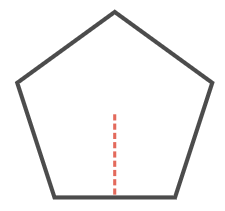
\includegraphics[width=0.6\linewidth]{../images/apotema.png}
    \end{figure}
        Si un polígono regular de $n$ lados, de longitud L, un perímetro de $P$ unidades, un apotema de $a$ unidades, entonces el área $A$ en unidades cuadradas es:
        \[A=\dfrac{nLa}{2}\]
        donde el perímetro es \[P=nL\]
\end{infocard}
